\documentclass[twoside]{book}

% Packages required by doxygen
\usepackage{fixltx2e}
\usepackage{calc}
\usepackage{doxygen}
\usepackage[export]{adjustbox} % also loads graphicx
\usepackage{graphicx}
\usepackage[utf8]{inputenc}
\usepackage{makeidx}
\usepackage{multicol}
\usepackage{multirow}
\PassOptionsToPackage{warn}{textcomp}
\usepackage{textcomp}
\usepackage[nointegrals]{wasysym}
\usepackage[table]{xcolor}

% Font selection
\usepackage[T1]{fontenc}
\usepackage[scaled=.90]{helvet}
\usepackage{courier}
\usepackage{amssymb}
\usepackage{sectsty}
\renewcommand{\familydefault}{\sfdefault}
\allsectionsfont{%
  \fontseries{bc}\selectfont%
  \color{darkgray}%
}
\renewcommand{\DoxyLabelFont}{%
  \fontseries{bc}\selectfont%
  \color{darkgray}%
}
\newcommand{\+}{\discretionary{\mbox{\scriptsize$\hookleftarrow$}}{}{}}

% Page & text layout
\usepackage{geometry}
\geometry{%
  a4paper,%
  top=2.5cm,%
  bottom=2.5cm,%
  left=2.5cm,%
  right=2.5cm%
}
\tolerance=750
\hfuzz=15pt
\hbadness=750
\setlength{\emergencystretch}{15pt}
\setlength{\parindent}{0cm}
\setlength{\parskip}{3ex plus 2ex minus 2ex}
\makeatletter
\renewcommand{\paragraph}{%
  \@startsection{paragraph}{4}{0ex}{-1.0ex}{1.0ex}{%
    \normalfont\normalsize\bfseries\SS@parafont%
  }%
}
\renewcommand{\subparagraph}{%
  \@startsection{subparagraph}{5}{0ex}{-1.0ex}{1.0ex}{%
    \normalfont\normalsize\bfseries\SS@subparafont%
  }%
}
\makeatother

% Headers & footers
\usepackage{fancyhdr}
\pagestyle{fancyplain}
\fancyhead[LE]{\fancyplain{}{\bfseries\thepage}}
\fancyhead[CE]{\fancyplain{}{}}
\fancyhead[RE]{\fancyplain{}{\bfseries\leftmark}}
\fancyhead[LO]{\fancyplain{}{\bfseries\rightmark}}
\fancyhead[CO]{\fancyplain{}{}}
\fancyhead[RO]{\fancyplain{}{\bfseries\thepage}}
\fancyfoot[LE]{\fancyplain{}{}}
\fancyfoot[CE]{\fancyplain{}{}}
\fancyfoot[RE]{\fancyplain{}{\bfseries\scriptsize Generated by Doxygen }}
\fancyfoot[LO]{\fancyplain{}{\bfseries\scriptsize Generated by Doxygen }}
\fancyfoot[CO]{\fancyplain{}{}}
\fancyfoot[RO]{\fancyplain{}{}}
\renewcommand{\footrulewidth}{0.4pt}
\renewcommand{\chaptermark}[1]{%
  \markboth{#1}{}%
}
\renewcommand{\sectionmark}[1]{%
  \markright{\thesection\ #1}%
}

% Indices & bibliography
\usepackage{natbib}
\usepackage[titles]{tocloft}
\setcounter{tocdepth}{3}
\setcounter{secnumdepth}{5}
\makeindex

% Hyperlinks (required, but should be loaded last)
\usepackage{ifpdf}
\ifpdf
  \usepackage[pdftex,pagebackref=true]{hyperref}
\else
  \usepackage[ps2pdf,pagebackref=true]{hyperref}
\fi
\hypersetup{%
  colorlinks=true,%
  linkcolor=blue,%
  citecolor=blue,%
  unicode%
}

% Custom commands
\newcommand{\clearemptydoublepage}{%
  \newpage{\pagestyle{empty}\cleardoublepage}%
}

\usepackage{caption}
\captionsetup{labelsep=space,justification=centering,font={bf},singlelinecheck=off,skip=4pt,position=top}

%===== C O N T E N T S =====

\begin{document}

% Titlepage & ToC
\hypersetup{pageanchor=false,
             bookmarksnumbered=true,
             pdfencoding=unicode
            }
\pagenumbering{alph}
\begin{titlepage}
\vspace*{7cm}
\begin{center}%
{\Large My Project }\\
\vspace*{1cm}
{\large Generated by Doxygen 1.8.13}\\
\end{center}
\end{titlepage}
\clearemptydoublepage
\pagenumbering{roman}
\tableofcontents
\clearemptydoublepage
\pagenumbering{arabic}
\hypersetup{pageanchor=true}

%--- Begin generated contents ---
\chapter{Space\+\_\+\+Invaders}
\label{autotoc_md0}
\Hypertarget{autotoc_md0}
Todo\+:~\newline
~\newline
 Optimaliseren transX en transY(enum?)~\newline
 M\+VC Abstract inhertince nuttig? of is Entity genoeg~\newline
 Texture class member view?~\newline
 Tex niet maken rechtstreeks memberclasses texture aanroepen~\newline
 playership foto scale size?~\newline
 
\chapter{Hierarchical Index}
\doxysection{Class Hierarchy}
This inheritance list is sorted roughly, but not completely, alphabetically\+:\begin{DoxyCompactList}
\item \contentsline{section}{Controller\+Abstract}{\pageref{classControllerAbstract}}{}
\begin{DoxyCompactList}
\item \contentsline{section}{Entity\+::Entity\+Controller}{\pageref{classEntity_1_1EntityController}}{}
\begin{DoxyCompactList}
\item \contentsline{section}{Entity\+::Collidable\+Controller}{\pageref{classEntity_1_1CollidableController}}{}
\begin{DoxyCompactList}
\item \contentsline{section}{Entity\+::Alive\+Controller}{\pageref{classEntity_1_1AliveController}}{}
\begin{DoxyCompactList}
\item \contentsline{section}{Entity\+::Enemy\+Controller}{\pageref{classEntity_1_1EnemyController}}{}
\begin{DoxyCompactList}
\item \contentsline{section}{Entity\+::Alien\+Ship\+Controller}{\pageref{classEntity_1_1AlienShipController}}{}
\end{DoxyCompactList}
\item \contentsline{section}{Entity\+::Player\+Ship\+Controller}{\pageref{classEntity_1_1PlayerShipController}}{}
\end{DoxyCompactList}
\item \contentsline{section}{Entity\+::Bullet\+Controller}{\pageref{classEntity_1_1BulletController}}{}
\item \contentsline{section}{Entity\+::Shield\+Controller}{\pageref{classEntity_1_1ShieldController}}{}
\end{DoxyCompactList}
\end{DoxyCompactList}
\end{DoxyCompactList}
\item enable\+\_\+shared\+\_\+from\+\_\+this\begin{DoxyCompactList}
\item \contentsline{section}{Entity\+::Bullet\+Controller}{\pageref{classEntity_1_1BulletController}}{}
\item \contentsline{section}{Entity\+::Enemy\+Controller}{\pageref{classEntity_1_1EnemyController}}{}
\end{DoxyCompactList}
\item \contentsline{section}{Game}{\pageref{classGame}}{}
\item \contentsline{section}{Utils\+::Object}{\pageref{structUtils_1_1Object}}{}
\item \contentsline{section}{Utils\+::Object\+Manager}{\pageref{classUtils_1_1ObjectManager}}{}
\item \contentsline{section}{Observer}{\pageref{classObserver}}{}
\begin{DoxyCompactList}
\item \contentsline{section}{View\+Abstract}{\pageref{classViewAbstract}}{}
\begin{DoxyCompactList}
\item \contentsline{section}{Entity\+::Entity\+View}{\pageref{classEntity_1_1EntityView}}{}
\begin{DoxyCompactList}
\item \contentsline{section}{Entity\+::Alien\+Ship\+View}{\pageref{classEntity_1_1AlienShipView}}{}
\item \contentsline{section}{Entity\+::Bullet\+View}{\pageref{classEntity_1_1BulletView}}{}
\item \contentsline{section}{Entity\+::Life\+View}{\pageref{classEntity_1_1LifeView}}{}
\item \contentsline{section}{Entity\+::Player\+Score\+View}{\pageref{classEntity_1_1PlayerScoreView}}{}
\item \contentsline{section}{Entity\+::Player\+Ship\+View}{\pageref{classEntity_1_1PlayerShipView}}{}
\item \contentsline{section}{Entity\+::Shield\+View}{\pageref{classEntity_1_1ShieldView}}{}
\end{DoxyCompactList}
\end{DoxyCompactList}
\end{DoxyCompactList}
\item \contentsline{section}{Utils\+::Stop\+Watch}{\pageref{classUtils_1_1StopWatch}}{}
\item \contentsline{section}{Subject}{\pageref{classSubject}}{}
\begin{DoxyCompactList}
\item \contentsline{section}{Model\+Abstract}{\pageref{classModelAbstract}}{}
\begin{DoxyCompactList}
\item \contentsline{section}{Entity\+::Entity\+Model}{\pageref{classEntity_1_1EntityModel}}{}
\begin{DoxyCompactList}
\item \contentsline{section}{Entity\+::Alive\+Model}{\pageref{classEntity_1_1AliveModel}}{}
\begin{DoxyCompactList}
\item \contentsline{section}{Entity\+::Enemy\+Model}{\pageref{classEntity_1_1EnemyModel}}{}
\begin{DoxyCompactList}
\item \contentsline{section}{Entity\+::Alien\+Ship\+Model}{\pageref{classEntity_1_1AlienShipModel}}{}
\end{DoxyCompactList}
\item \contentsline{section}{Entity\+::Player\+Ship\+Model}{\pageref{classEntity_1_1PlayerShipModel}}{}
\end{DoxyCompactList}
\item \contentsline{section}{Entity\+::Bullet\+Model}{\pageref{classEntity_1_1BulletModel}}{}
\item \contentsline{section}{Entity\+::Shield\+Model}{\pageref{classEntity_1_1ShieldModel}}{}
\end{DoxyCompactList}
\end{DoxyCompactList}
\end{DoxyCompactList}
\item \contentsline{section}{Utils\+::Transformation}{\pageref{classUtils_1_1Transformation}}{}
\item \contentsline{section}{Utils\+::Vector2D}{\pageref{structUtils_1_1Vector2D}}{}
\end{DoxyCompactList}

\chapter{Class Index}
\doxysection{Class List}
Here are the classes, structs, unions and interfaces with brief descriptions\+:\begin{DoxyCompactList}
\item\contentsline{section}{\mbox{\hyperlink{classEntity_1_1AlienShipController}{Entity\+::\+Alien\+Ship\+Controller}} }{\pageref{classEntity_1_1AlienShipController}}{}
\item\contentsline{section}{\mbox{\hyperlink{classEntity_1_1AlienShipModel}{Entity\+::\+Alien\+Ship\+Model}} }{\pageref{classEntity_1_1AlienShipModel}}{}
\item\contentsline{section}{\mbox{\hyperlink{classEntity_1_1AlienShipView}{Entity\+::\+Alien\+Ship\+View}} }{\pageref{classEntity_1_1AlienShipView}}{}
\item\contentsline{section}{\mbox{\hyperlink{classEntity_1_1AliveController}{Entity\+::\+Alive\+Controller}} }{\pageref{classEntity_1_1AliveController}}{}
\item\contentsline{section}{\mbox{\hyperlink{classEntity_1_1AliveModel}{Entity\+::\+Alive\+Model}} }{\pageref{classEntity_1_1AliveModel}}{}
\item\contentsline{section}{\mbox{\hyperlink{classEntity_1_1BulletController}{Entity\+::\+Bullet\+Controller}} }{\pageref{classEntity_1_1BulletController}}{}
\item\contentsline{section}{\mbox{\hyperlink{classEntity_1_1BulletModel}{Entity\+::\+Bullet\+Model}} }{\pageref{classEntity_1_1BulletModel}}{}
\item\contentsline{section}{\mbox{\hyperlink{classEntity_1_1BulletView}{Entity\+::\+Bullet\+View}} }{\pageref{classEntity_1_1BulletView}}{}
\item\contentsline{section}{\mbox{\hyperlink{classEntity_1_1CollidableController}{Entity\+::\+Collidable\+Controller}} }{\pageref{classEntity_1_1CollidableController}}{}
\item\contentsline{section}{\mbox{\hyperlink{classControllerAbstract}{Controller\+Abstract}} }{\pageref{classControllerAbstract}}{}
\item\contentsline{section}{\mbox{\hyperlink{classEntity_1_1EnemyController}{Entity\+::\+Enemy\+Controller}} }{\pageref{classEntity_1_1EnemyController}}{}
\item\contentsline{section}{\mbox{\hyperlink{classEntity_1_1EnemyModel}{Entity\+::\+Enemy\+Model}} }{\pageref{classEntity_1_1EnemyModel}}{}
\item\contentsline{section}{\mbox{\hyperlink{classEntity_1_1EntityController}{Entity\+::\+Entity\+Controller}} }{\pageref{classEntity_1_1EntityController}}{}
\item\contentsline{section}{\mbox{\hyperlink{classEntity_1_1EntityModel}{Entity\+::\+Entity\+Model}} \\*Model class for Entity this class handles all the data of Entity }{\pageref{classEntity_1_1EntityModel}}{}
\item\contentsline{section}{\mbox{\hyperlink{classEntity_1_1EntityView}{Entity\+::\+Entity\+View}} \\*View class for Entity this class handles the visual aspect of the game }{\pageref{classEntity_1_1EntityView}}{}
\item\contentsline{section}{\mbox{\hyperlink{classGame}{Game}} }{\pageref{classGame}}{}
\item\contentsline{section}{\mbox{\hyperlink{classEntity_1_1LifeView}{Entity\+::\+Life\+View}} }{\pageref{classEntity_1_1LifeView}}{}
\item\contentsline{section}{\mbox{\hyperlink{classModelAbstract}{Model\+Abstract}} \\*Superclass of all model classes handles the data section of the game }{\pageref{classModelAbstract}}{}
\item\contentsline{section}{\mbox{\hyperlink{structUtils_1_1Object}{Utils\+::\+Object}} }{\pageref{structUtils_1_1Object}}{}
\item\contentsline{section}{\mbox{\hyperlink{classUtils_1_1ObjectManager}{Utils\+::\+Object\+Manager}} }{\pageref{classUtils_1_1ObjectManager}}{}
\item\contentsline{section}{\mbox{\hyperlink{classObserver}{Observer}} }{\pageref{classObserver}}{}
\item\contentsline{section}{\mbox{\hyperlink{classEntity_1_1PlayerScoreView}{Entity\+::\+Player\+Score\+View}} }{\pageref{classEntity_1_1PlayerScoreView}}{}
\item\contentsline{section}{\mbox{\hyperlink{classEntity_1_1PlayerShipController}{Entity\+::\+Player\+Ship\+Controller}} }{\pageref{classEntity_1_1PlayerShipController}}{}
\item\contentsline{section}{\mbox{\hyperlink{classEntity_1_1PlayerShipModel}{Entity\+::\+Player\+Ship\+Model}} \\*Model of the Player\+Ship handles all the data for Player\+Ship }{\pageref{classEntity_1_1PlayerShipModel}}{}
\item\contentsline{section}{\mbox{\hyperlink{classEntity_1_1PlayerShipView}{Entity\+::\+Player\+Ship\+View}} \\*View class for Player\+Ship this class handles the visual aspect of the game }{\pageref{classEntity_1_1PlayerShipView}}{}
\item\contentsline{section}{\mbox{\hyperlink{classUtils_1_1StopWatch}{Utils\+::\+Stop\+Watch}} }{\pageref{classUtils_1_1StopWatch}}{}
\item\contentsline{section}{\mbox{\hyperlink{classSubject}{Subject}} }{\pageref{classSubject}}{}
\item\contentsline{section}{\mbox{\hyperlink{classUtils_1_1Transformation}{Utils\+::\+Transformation}} \\*Used for transforming a models x and y values to the corresponding values on the screen }{\pageref{classUtils_1_1Transformation}}{}
\item\contentsline{section}{\mbox{\hyperlink{structUtils_1_1Vector2D}{Utils\+::\+Vector2D}} }{\pageref{structUtils_1_1Vector2D}}{}
\item\contentsline{section}{\mbox{\hyperlink{classViewAbstract}{View\+Abstract}} \\*Superclass of all view classes handles the visual aspect of the game }{\pageref{classViewAbstract}}{}
\end{DoxyCompactList}

\chapter{Class Documentation}
\hypertarget{classControllable}{}\section{Controllable Class Reference}
\label{classControllable}\index{Controllable@{Controllable}}
Inheritance diagram for Controllable\+:\begin{figure}[H]
\begin{center}
\leavevmode
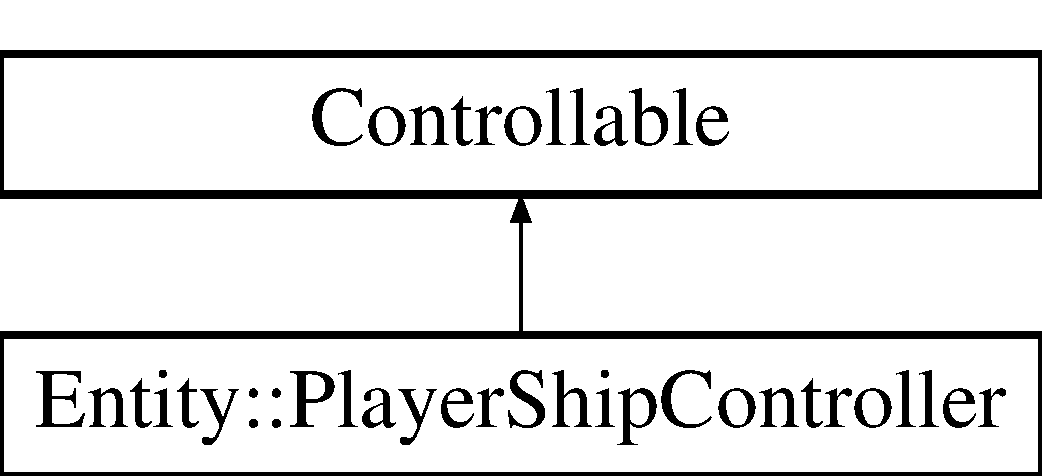
\includegraphics[height=2.000000cm]{classControllable}
\end{center}
\end{figure}


\subsection{Detailed Description}


Definition at line 8 of file Controllable.\+h.



The documentation for this class was generated from the following file\+:\begin{DoxyCompactItemize}
\item 
M\+V\+C\+Abstract/Controllable.\+h\end{DoxyCompactItemize}

\hypertarget{classControllerAbstract}{}\doxysection{Controller\+Abstract Class Reference}
\label{classControllerAbstract}\index{ControllerAbstract@{ControllerAbstract}}
Inheritance diagram for Controller\+Abstract\+:\begin{figure}[H]
\begin{center}
\leavevmode
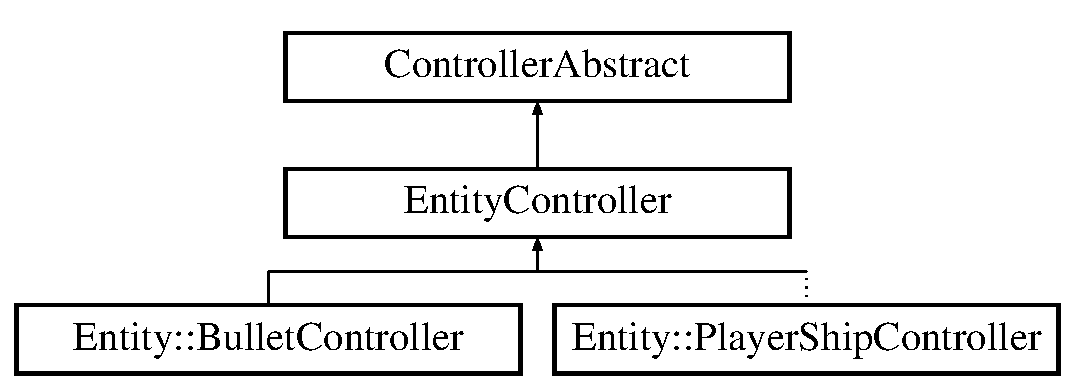
\includegraphics[height=3.000000cm]{classControllerAbstract}
\end{center}
\end{figure}
\doxysubsection*{Public Member Functions}
\begin{DoxyCompactItemize}
\item 
\mbox{\Hypertarget{classControllerAbstract_a9ff7d37a76409a65aed7870458b13e5c}\label{classControllerAbstract_a9ff7d37a76409a65aed7870458b13e5c}} 
{\bfseries Controller\+Abstract} (const std\+::shared\+\_\+ptr$<$ \mbox{\hyperlink{classModelAbstract}{Model\+Abstract}} $>$ \&m, const std\+::shared\+\_\+ptr$<$ \mbox{\hyperlink{classViewAbstract}{View\+Abstract}} $>$ \&v)
\end{DoxyCompactItemize}
\doxysubsection*{Protected Attributes}
\begin{DoxyCompactItemize}
\item 
\mbox{\Hypertarget{classControllerAbstract_a9e02164cdd086533e3fd67bdbdce1d5b}\label{classControllerAbstract_a9e02164cdd086533e3fd67bdbdce1d5b}} 
std\+::shared\+\_\+ptr$<$ \mbox{\hyperlink{classModelAbstract}{Model\+Abstract}} $>$ {\bfseries m}
\item 
\mbox{\Hypertarget{classControllerAbstract_aeb469f80fa4b819b8922e63a9928d1ad}\label{classControllerAbstract_aeb469f80fa4b819b8922e63a9928d1ad}} 
std\+::shared\+\_\+ptr$<$ \mbox{\hyperlink{classViewAbstract}{View\+Abstract}} $>$ {\bfseries v}
\end{DoxyCompactItemize}


\doxysubsection{Detailed Description}


Definition at line 11 of file Controller\+Abstract.\+h.



The documentation for this class was generated from the following files\+:\begin{DoxyCompactItemize}
\item 
M\+V\+C\+Abstract/Controller\+Abstract.\+h\item 
M\+V\+C\+Abstract/Controller\+Abstract.\+cpp\end{DoxyCompactItemize}

\hypertarget{classEntity_1_1EnemyShipView}{}\doxysection{Entity\+::Enemy\+Ship\+View Class Reference}
\label{classEntity_1_1EnemyShipView}\index{Entity::EnemyShipView@{Entity::EnemyShipView}}


View class for Player\+Ship this class handles the visual aspect of the game.  




{\ttfamily \#include $<$Enemy\+Ship\+View.\+h$>$}

Inheritance diagram for Entity\+::Enemy\+Ship\+View\+:\begin{figure}[H]
\begin{center}
\leavevmode
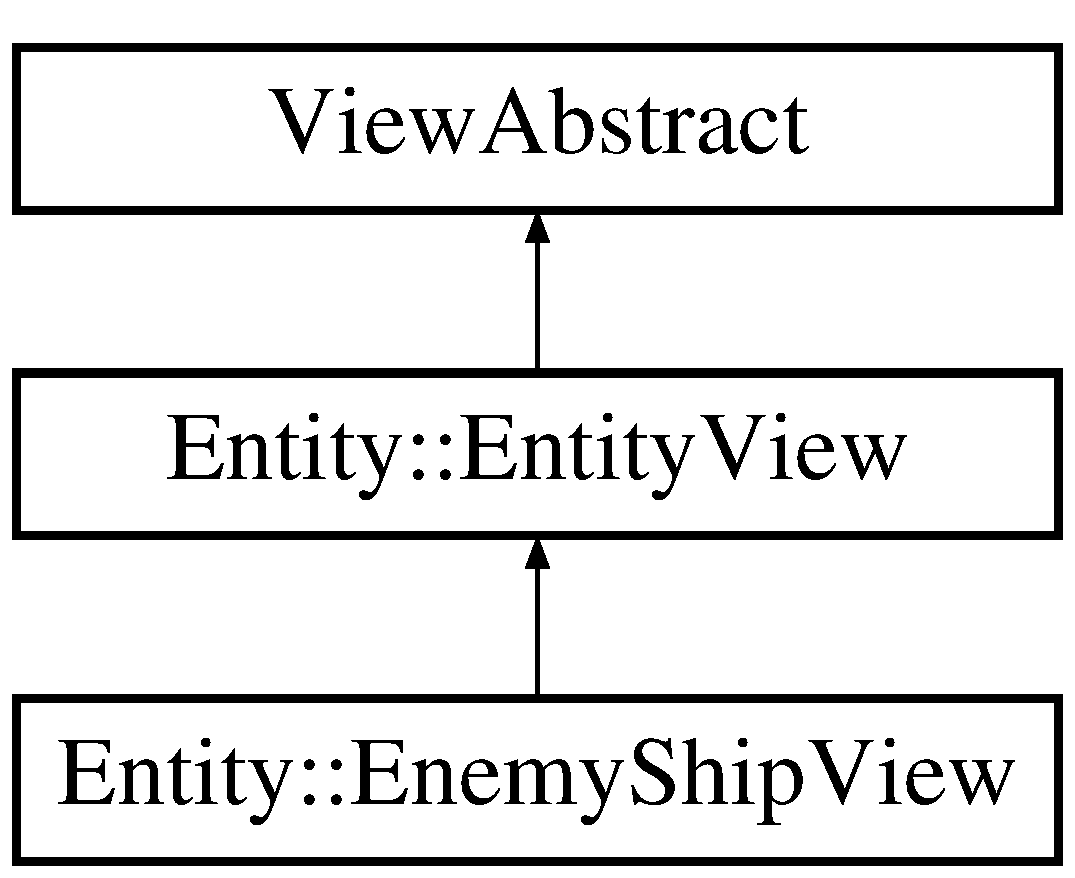
\includegraphics[height=3.000000cm]{classEntity_1_1EnemyShipView}
\end{center}
\end{figure}
\doxysubsection*{Public Member Functions}
\begin{DoxyCompactItemize}
\item 
void \mbox{\hyperlink{classEntity_1_1EnemyShipView_a3417632d012f12720ebbbe4b525b3c19}{draw}} (sf\+::\+Render\+Window \&w)
\begin{DoxyCompactList}\small\item\em draws the shape on the sf\+::\+Render\+Window w \end{DoxyCompactList}\item 
\mbox{\Hypertarget{classEntity_1_1EnemyShipView_a208188bb32ba97acefdd236227b223e6}\label{classEntity_1_1EnemyShipView_a208188bb32ba97acefdd236227b223e6}} 
\mbox{\hyperlink{classEntity_1_1EnemyShipView_a208188bb32ba97acefdd236227b223e6}{Enemy\+Ship\+View}} ()
\begin{DoxyCompactList}\small\item\em basic contructor for playership sets the shape to the standard square \end{DoxyCompactList}\item 
\mbox{\Hypertarget{classEntity_1_1EnemyShipView_ac023c3cd83fbc0ad66fa8221b006519b}\label{classEntity_1_1EnemyShipView_ac023c3cd83fbc0ad66fa8221b006519b}} 
void {\bfseries generate\+Shape} ()
\end{DoxyCompactItemize}


\doxysubsection{Detailed Description}
View class for Player\+Ship this class handles the visual aspect of the game. 

Definition at line 13 of file Enemy\+Ship\+View.\+h.



\doxysubsection{Member Function Documentation}
\mbox{\Hypertarget{classEntity_1_1EnemyShipView_a3417632d012f12720ebbbe4b525b3c19}\label{classEntity_1_1EnemyShipView_a3417632d012f12720ebbbe4b525b3c19}} 
\index{Entity::EnemyShipView@{Entity::EnemyShipView}!draw@{draw}}
\index{draw@{draw}!Entity::EnemyShipView@{Entity::EnemyShipView}}
\doxysubsubsection{\texorpdfstring{draw()}{draw()}}
{\footnotesize\ttfamily void Entity\+::\+Enemy\+Ship\+View\+::draw (\begin{DoxyParamCaption}\item[{sf\+::\+Render\+Window \&}]{w }\end{DoxyParamCaption})\hspace{0.3cm}{\ttfamily [virtual]}}



draws the shape on the sf\+::\+Render\+Window w 


\begin{DoxyParams}{Parameters}
{\em w} & the window where the shape gets drawn on. \\
\hline
\end{DoxyParams}


Implements \mbox{\hyperlink{classEntity_1_1EntityView_a9a415b467798f8bbb9cd2489c3edd941}{Entity\+::\+Entity\+View}}.



Definition at line 7 of file Enemy\+Ship\+View.\+cpp.


\begin{DoxyCode}{0}
\DoxyCodeLine{7 \{ w.draw(\mbox{\hyperlink{classEntity_1_1EntityView_a3902b7f2a7fb36363a227d59b7044e5a}{getShape}}()); \}}

\end{DoxyCode}


The documentation for this class was generated from the following files\+:\begin{DoxyCompactItemize}
\item 
Entity/\+Enemy\+Ship/Enemy\+Ship\+View.\+h\item 
Entity/\+Enemy\+Ship/Enemy\+Ship\+View.\+cpp\end{DoxyCompactItemize}

\hypertarget{classEntity_1_1EntityModel}{}\doxysection{Entity\+::Entity\+Model Class Reference}
\label{classEntity_1_1EntityModel}\index{Entity::EntityModel@{Entity::EntityModel}}


Model class for Entity this class handles all the data of Entity.  




{\ttfamily \#include $<$Entity\+Model.\+h$>$}

Inheritance diagram for Entity\+::Entity\+Model\+:\begin{figure}[H]
\begin{center}
\leavevmode
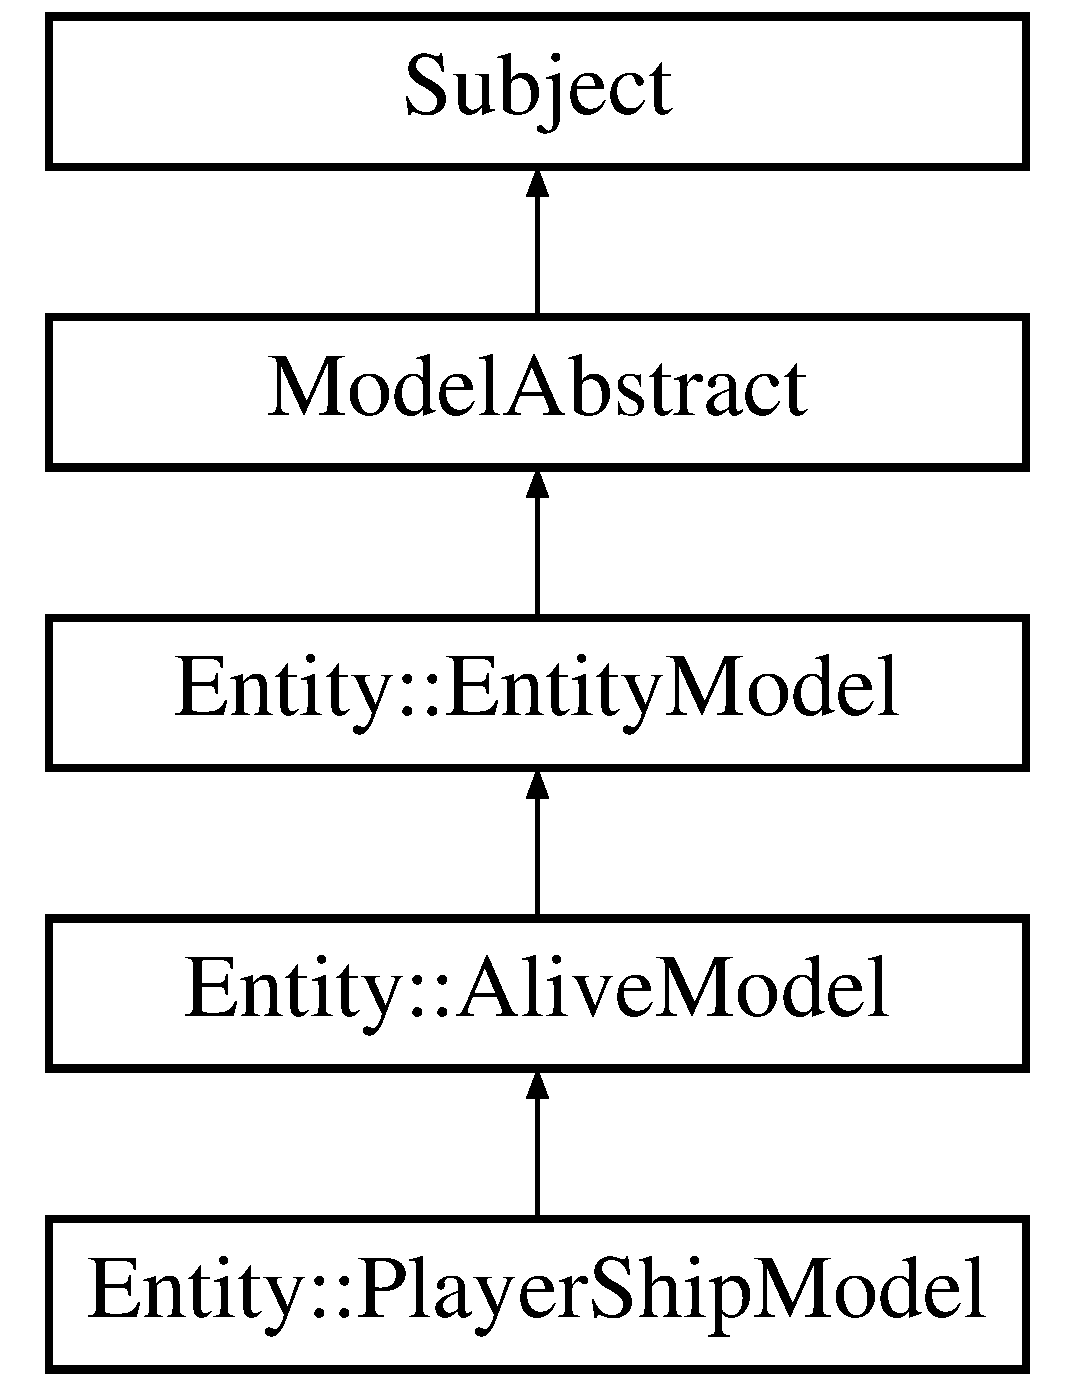
\includegraphics[height=6.000000cm]{classEntity_1_1EntityModel}
\end{center}
\end{figure}
\doxysubsection*{Public Member Functions}
\begin{DoxyCompactItemize}
\item 
\mbox{\Hypertarget{classEntity_1_1EntityModel_a14667d01eef84af4dfbbb9c6aea7c701}\label{classEntity_1_1EntityModel_a14667d01eef84af4dfbbb9c6aea7c701}} 
const \mbox{\hyperlink{structUtils_1_1Vector2D}{Utils\+::\+Vector2D}} \& {\bfseries get\+Size} () const
\item 
\mbox{\Hypertarget{classEntity_1_1EntityModel_a557817a4eef083aa0604876c22ac1a57}\label{classEntity_1_1EntityModel_a557817a4eef083aa0604876c22ac1a57}} 
void {\bfseries set\+Size} (const \mbox{\hyperlink{structUtils_1_1Vector2D}{Utils\+::\+Vector2D}} \&size)
\item 
\mbox{\Hypertarget{classEntity_1_1EntityModel_add95685f6c22f2e5e851089a3501f2ee}\label{classEntity_1_1EntityModel_add95685f6c22f2e5e851089a3501f2ee}} 
bool {\bfseries valid\+Position} (\mbox{\hyperlink{structUtils_1_1Vector2D}{Utils\+::\+Vector2D}})
\item 
\mbox{\Hypertarget{classEntity_1_1EntityModel_afd198901a1ad8c64361ced938d199494}\label{classEntity_1_1EntityModel_afd198901a1ad8c64361ced938d199494}} 
const \mbox{\hyperlink{structUtils_1_1Vector2D}{Utils\+::\+Vector2D}} \& {\bfseries get\+Position} () const
\item 
void \mbox{\hyperlink{classEntity_1_1EntityModel_a5cb470f2afae411ad0ee18ff7585d980}{notify\+Observers}} ()
\item 
\mbox{\Hypertarget{classEntity_1_1EntityModel_a027cb5db3c6bf8df5f761d7a69d35afe}\label{classEntity_1_1EntityModel_a027cb5db3c6bf8df5f761d7a69d35afe}} 
{\bfseries Entity\+Model} (const \mbox{\hyperlink{structUtils_1_1Vector2D}{Utils\+::\+Vector2D}} \&position, const \mbox{\hyperlink{structUtils_1_1Vector2D}{Utils\+::\+Vector2D}} \&size)
\end{DoxyCompactItemize}
\doxysubsection*{Protected Member Functions}
\begin{DoxyCompactItemize}
\item 
\mbox{\Hypertarget{classEntity_1_1EntityModel_a7f8964ced9ede24806efc18a88be658e}\label{classEntity_1_1EntityModel_a7f8964ced9ede24806efc18a88be658e}} 
bool {\bfseries set\+Position} (const \mbox{\hyperlink{structUtils_1_1Vector2D}{Utils\+::\+Vector2D}} \&position)
\end{DoxyCompactItemize}
\doxysubsection*{Protected Attributes}
\begin{DoxyCompactItemize}
\item 
\mbox{\Hypertarget{classEntity_1_1EntityModel_a38c2a78548aea09a5feeb1fb5c7d47e4}\label{classEntity_1_1EntityModel_a38c2a78548aea09a5feeb1fb5c7d47e4}} 
\mbox{\hyperlink{structUtils_1_1Vector2D}{Utils\+::\+Vector2D}} {\bfseries position}
\item 
\mbox{\Hypertarget{classEntity_1_1EntityModel_ad0997b52258cb8903d1d2a6bfdbbb770}\label{classEntity_1_1EntityModel_ad0997b52258cb8903d1d2a6bfdbbb770}} 
\mbox{\hyperlink{structUtils_1_1Vector2D}{Utils\+::\+Vector2D}} {\bfseries size}
\end{DoxyCompactItemize}


\doxysubsection{Detailed Description}
Model class for Entity this class handles all the data of Entity. 

Definition at line 13 of file Entity\+Model.\+h.



\doxysubsection{Member Function Documentation}
\mbox{\Hypertarget{classEntity_1_1EntityModel_a5cb470f2afae411ad0ee18ff7585d980}\label{classEntity_1_1EntityModel_a5cb470f2afae411ad0ee18ff7585d980}} 
\index{Entity::EntityModel@{Entity::EntityModel}!notifyObservers@{notifyObservers}}
\index{notifyObservers@{notifyObservers}!Entity::EntityModel@{Entity::EntityModel}}
\doxysubsubsection{\texorpdfstring{notifyObservers()}{notifyObservers()}}
{\footnotesize\ttfamily void Entity\+::\+Entity\+Model\+::notify\+Observers (\begin{DoxyParamCaption}{ }\end{DoxyParamCaption})\hspace{0.3cm}{\ttfamily [virtual]}}

the contrustructor of \mbox{\hyperlink{classEntity_1_1EntityModel}{Entity\+Model}} creates a Entity with healthpoints, x\+Val, Yval 
\begin{DoxyParams}{Parameters}
{\em health\+Points} & The health\+Points of the Entity \\
\hline
{\em x\+Val} & The x\+Val of the Entity \\
\hline
{\em Yval} & The y\+Val of the Entity \\
\hline
\end{DoxyParams}


Implements \mbox{\hyperlink{classSubject}{Subject}}.



Definition at line 8 of file Entity\+Model.\+cpp.


\begin{DoxyCode}{0}
\DoxyCodeLine{9 \{}
\DoxyCodeLine{10         \textcolor{keywordflow}{for} (\textcolor{keywordtype}{int} i = 0; i < observers.size(); ++i) \{}
\DoxyCodeLine{11                 observers[i]-\/>update();}
\DoxyCodeLine{12         \}}
\DoxyCodeLine{13 \}}

\end{DoxyCode}


The documentation for this class was generated from the following files\+:\begin{DoxyCompactItemize}
\item 
Entity/Entity\+Model.\+h\item 
Entity/Entity\+Model.\+cpp\end{DoxyCompactItemize}

\hypertarget{classEntity_1_1EntityView}{}\doxysection{Entity\+::Entity\+View Class Reference}
\label{classEntity_1_1EntityView}\index{Entity::EntityView@{Entity::EntityView}}


View class for Entity this class handles the visual aspect of the game.  




{\ttfamily \#include $<$Entity\+View.\+h$>$}

Inheritance diagram for Entity\+::Entity\+View\+:\begin{figure}[H]
\begin{center}
\leavevmode
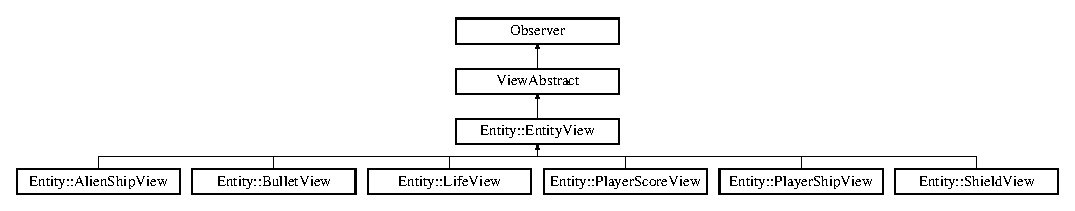
\includegraphics[height=3.000000cm]{classEntity_1_1EntityView}
\end{center}
\end{figure}
\doxysubsection*{Public Member Functions}
\begin{DoxyCompactItemize}
\item 
\mbox{\Hypertarget{classEntity_1_1EntityView_abd5ed0dd272fc216f201020b2ac4e8b1}\label{classEntity_1_1EntityView_abd5ed0dd272fc216f201020b2ac4e8b1}} 
double {\bfseries get\+Size} () const
\item 
\mbox{\Hypertarget{classEntity_1_1EntityView_afa0c120d100bad7f62b240beadfcee02}\label{classEntity_1_1EntityView_afa0c120d100bad7f62b240beadfcee02}} 
void {\bfseries set\+Size} (double size)
\item 
\mbox{\Hypertarget{classEntity_1_1EntityView_a2e9bf31d4e90ab92b8ad5d96f2057846}\label{classEntity_1_1EntityView_a2e9bf31d4e90ab92b8ad5d96f2057846}} 
const sf\+::\+Texture \& {\bfseries get\+Texture} () const
\item 
\mbox{\Hypertarget{classEntity_1_1EntityView_aed6c61089c3d8de22bbe895e69d901b5}\label{classEntity_1_1EntityView_aed6c61089c3d8de22bbe895e69d901b5}} 
void {\bfseries set\+Texture} (const sf\+::\+Texture \&texture)
\item 
sf\+::\+Sprite \mbox{\hyperlink{classEntity_1_1EntityView_a3902b7f2a7fb36363a227d59b7044e5a}{get\+Shape}} () const
\item 
void \mbox{\hyperlink{classEntity_1_1EntityView_ab462f61f84150553ac1cf87c67f529f4}{set\+Shape}} (sf\+::\+Sprite shape)
\item 
virtual void \mbox{\hyperlink{classEntity_1_1EntityView_a9a415b467798f8bbb9cd2489c3edd941}{draw}} (sf\+::\+Render\+Window \&w)=0
\begin{DoxyCompactList}\small\item\em draws the shape on the sf\+::\+Render\+Window w \end{DoxyCompactList}\item 
\mbox{\Hypertarget{classEntity_1_1EntityView_aa7ac759577e903d916b7f62e81acfc39}\label{classEntity_1_1EntityView_aa7ac759577e903d916b7f62e81acfc39}} 
void {\bfseries update} (double, double)
\item 
\mbox{\Hypertarget{classEntity_1_1EntityView_ae4aeb4a57034976467848d12906d3042}\label{classEntity_1_1EntityView_ae4aeb4a57034976467848d12906d3042}} 
virtual void {\bfseries generate\+Shape} ()=0
\end{DoxyCompactItemize}


\doxysubsection{Detailed Description}
View class for Entity this class handles the visual aspect of the game. 

Definition at line 14 of file Entity\+View.\+h.



\doxysubsection{Member Function Documentation}
\mbox{\Hypertarget{classEntity_1_1EntityView_a9a415b467798f8bbb9cd2489c3edd941}\label{classEntity_1_1EntityView_a9a415b467798f8bbb9cd2489c3edd941}} 
\index{Entity::EntityView@{Entity::EntityView}!draw@{draw}}
\index{draw@{draw}!Entity::EntityView@{Entity::EntityView}}
\doxysubsubsection{\texorpdfstring{draw()}{draw()}}
{\footnotesize\ttfamily virtual void Entity\+::\+Entity\+View\+::draw (\begin{DoxyParamCaption}\item[{sf\+::\+Render\+Window \&}]{w }\end{DoxyParamCaption})\hspace{0.3cm}{\ttfamily [pure virtual]}}



draws the shape on the sf\+::\+Render\+Window w 


\begin{DoxyParams}{Parameters}
{\em w} & the window where the shape gets drawn on. \\
\hline
\end{DoxyParams}


Implements \mbox{\hyperlink{classViewAbstract_ab9d21012b19948e704a800da39b232ba}{View\+Abstract}}.



Implemented in \mbox{\hyperlink{classEntity_1_1PlayerShipView_ad9767510af4af87a4b67182065a1bf6c}{Entity\+::\+Player\+Ship\+View}}, and \mbox{\hyperlink{classEntity_1_1EnemyShipView_a3417632d012f12720ebbbe4b525b3c19}{Entity\+::\+Enemy\+Ship\+View}}.

\mbox{\Hypertarget{classEntity_1_1EntityView_a3902b7f2a7fb36363a227d59b7044e5a}\label{classEntity_1_1EntityView_a3902b7f2a7fb36363a227d59b7044e5a}} 
\index{Entity::EntityView@{Entity::EntityView}!getShape@{getShape}}
\index{getShape@{getShape}!Entity::EntityView@{Entity::EntityView}}
\doxysubsubsection{\texorpdfstring{getShape()}{getShape()}}
{\footnotesize\ttfamily sf\+::\+Sprite Entity\+::\+Entity\+View\+::get\+Shape (\begin{DoxyParamCaption}{ }\end{DoxyParamCaption}) const}

returns the sf\+::drawable of this Entity \begin{DoxyReturn}{Returns}
const sf\+::\+Drawable of this Entity 
\end{DoxyReturn}


Definition at line 8 of file Entity\+View.\+cpp.


\begin{DoxyCode}{0}
\DoxyCodeLine{8 \{ \textcolor{keywordflow}{return} shape; \}}

\end{DoxyCode}
\mbox{\Hypertarget{classEntity_1_1EntityView_ab462f61f84150553ac1cf87c67f529f4}\label{classEntity_1_1EntityView_ab462f61f84150553ac1cf87c67f529f4}} 
\index{Entity::EntityView@{Entity::EntityView}!setShape@{setShape}}
\index{setShape@{setShape}!Entity::EntityView@{Entity::EntityView}}
\doxysubsubsection{\texorpdfstring{setShape()}{setShape()}}
{\footnotesize\ttfamily void Entity\+::\+Entity\+View\+::set\+Shape (\begin{DoxyParamCaption}\item[{sf\+::\+Sprite}]{shape }\end{DoxyParamCaption})}

sets the shape of this Entity to the given shape 
\begin{DoxyParams}{Parameters}
{\em shape} & the new shape of this Entity \\
\hline
\end{DoxyParams}


Definition at line 10 of file Entity\+View.\+cpp.


\begin{DoxyCode}{0}
\DoxyCodeLine{10 \{ EntityView::shape = shape; \}}

\end{DoxyCode}


The documentation for this class was generated from the following files\+:\begin{DoxyCompactItemize}
\item 
Entity/Entity\+View.\+h\item 
Entity/Entity\+View.\+cpp\end{DoxyCompactItemize}

\hypertarget{classModelAbstract}{}\doxysection{Model\+Abstract Class Reference}
\label{classModelAbstract}\index{ModelAbstract@{ModelAbstract}}


superclass of all model classes handles the data section of the game  




{\ttfamily \#include $<$Model\+Abstract.\+h$>$}

Inheritance diagram for Model\+Abstract\+:\begin{figure}[H]
\begin{center}
\leavevmode
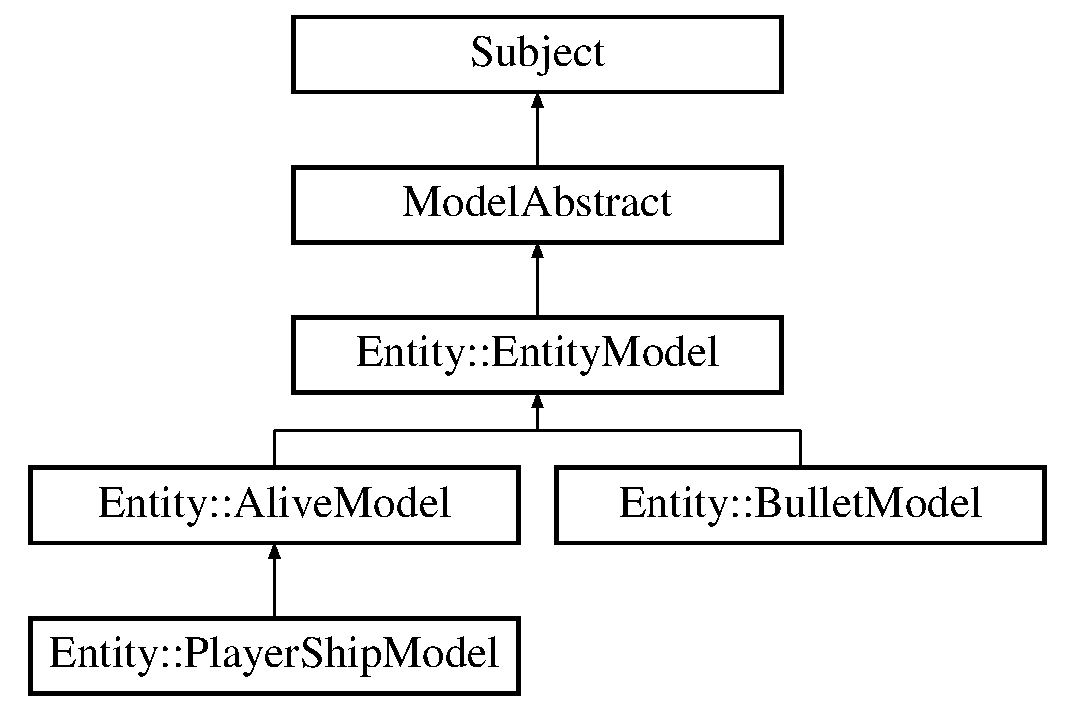
\includegraphics[height=5.000000cm]{classModelAbstract}
\end{center}
\end{figure}
\doxysubsection*{Additional Inherited Members}


\doxysubsection{Detailed Description}
superclass of all model classes handles the data section of the game 

Definition at line 12 of file Model\+Abstract.\+h.



The documentation for this class was generated from the following file\+:\begin{DoxyCompactItemize}
\item 
M\+V\+C\+Abstract/Model\+Abstract.\+h\end{DoxyCompactItemize}

\hypertarget{classObserver}{}\doxysection{Observer Class Reference}
\label{classObserver}\index{Observer@{Observer}}


the observer from the observerpattern  




{\ttfamily \#include $<$Observer.\+h$>$}

Inheritance diagram for Observer\+:\begin{figure}[H]
\begin{center}
\leavevmode
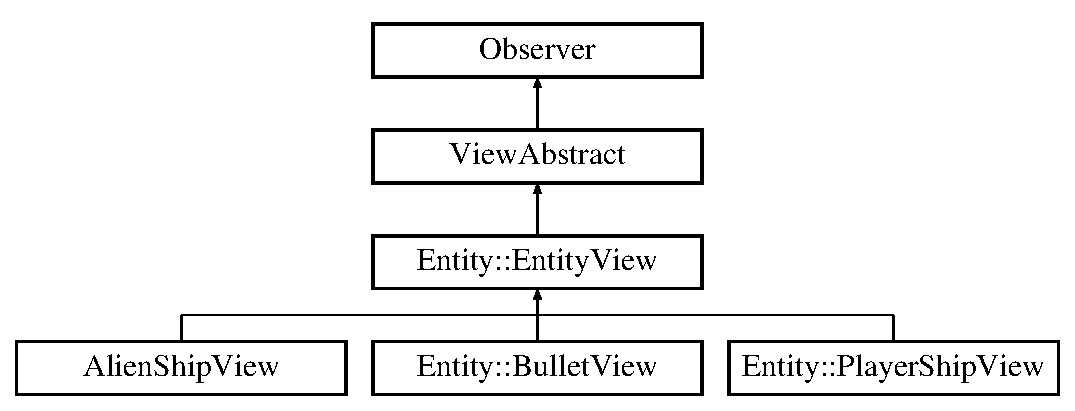
\includegraphics[height=2.393162cm]{classObserver}
\end{center}
\end{figure}
\doxysubsection*{Public Member Functions}
\begin{DoxyCompactItemize}
\item 
\mbox{\Hypertarget{classObserver_ac75e4b339faeb3ea6fe0a01bf0b4a215}\label{classObserver_ac75e4b339faeb3ea6fe0a01bf0b4a215}} 
virtual void \mbox{\hyperlink{classObserver_ac75e4b339faeb3ea6fe0a01bf0b4a215}{update}} ()=0
\begin{DoxyCompactList}\small\item\em gets called when the subject does notify observers this function is used for updating this class when the subject calls notifyobservers \end{DoxyCompactList}\end{DoxyCompactItemize}


\doxysubsection{Detailed Description}
the observer from the observerpattern 

Definition at line 11 of file Observer.\+h.



The documentation for this class was generated from the following file\+:\begin{DoxyCompactItemize}
\item 
Observer/Observer.\+h\end{DoxyCompactItemize}

\hypertarget{classEntity_1_1PlayerShipController}{}\section{Entity\+:\+:Player\+Ship\+Controller Class Reference}
\label{classEntity_1_1PlayerShipController}\index{Entity\+::\+Player\+Ship\+Controller@{Entity\+::\+Player\+Ship\+Controller}}
Inheritance diagram for Entity\+:\+:Player\+Ship\+Controller\+:\begin{figure}[H]
\begin{center}
\leavevmode
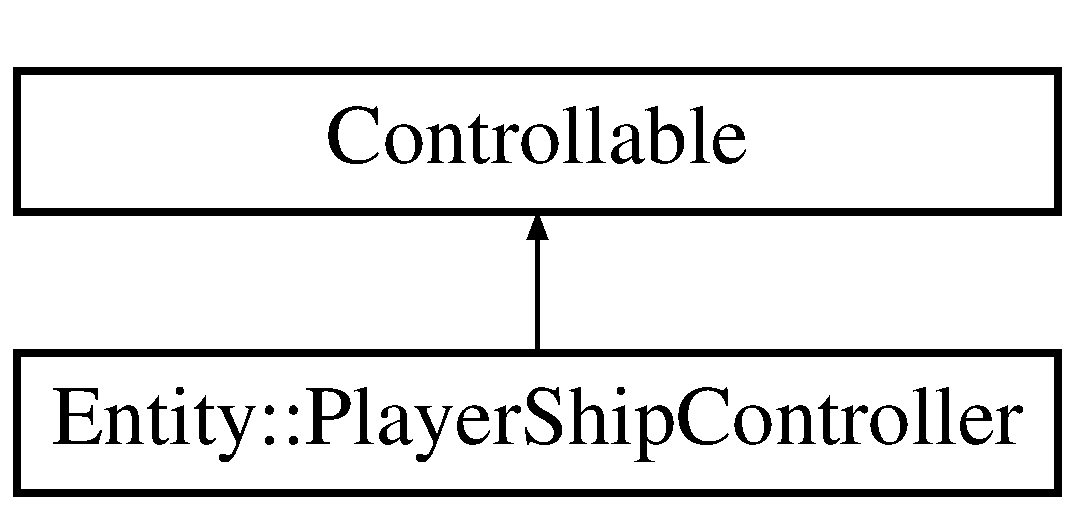
\includegraphics[height=2.000000cm]{classEntity_1_1PlayerShipController}
\end{center}
\end{figure}
\subsection*{Public Member Functions}
\begin{DoxyCompactItemize}
\item 
\mbox{\Hypertarget{classEntity_1_1PlayerShipController_a5bb5ec6d9262030be9375ffc8434c896}\label{classEntity_1_1PlayerShipController_a5bb5ec6d9262030be9375ffc8434c896}} 
void {\bfseries read\+Input} ()
\item 
\mbox{\Hypertarget{classEntity_1_1PlayerShipController_ac137389e2a1ba192ad747df7deac5c7c}\label{classEntity_1_1PlayerShipController_ac137389e2a1ba192ad747df7deac5c7c}} 
{\bfseries Player\+Ship\+Controller} (\hyperlink{classEntity_1_1PlayerShipModel}{Player\+Ship\+Model} $\ast$m, \hyperlink{classEntity_1_1PlayerShipView}{Player\+Ship\+View} $\ast$v)
\end{DoxyCompactItemize}


\subsection{Detailed Description}


Definition at line 14 of file Player\+Ship\+Controller.\+h.



The documentation for this class was generated from the following files\+:\begin{DoxyCompactItemize}
\item 
Entity/\+Player\+Ship/Player\+Ship\+Controller.\+h\item 
Entity/\+Player\+Ship/Player\+Ship\+Controller.\+cpp\end{DoxyCompactItemize}

\hypertarget{classEntity_1_1PlayerShipModel}{}\doxysection{Entity\+::Player\+Ship\+Model Class Reference}
\label{classEntity_1_1PlayerShipModel}\index{Entity::PlayerShipModel@{Entity::PlayerShipModel}}


Model of the Player\+Ship handles all the data for Player\+Ship.  




{\ttfamily \#include $<$Player\+Ship\+Model.\+h$>$}

Inheritance diagram for Entity\+::Player\+Ship\+Model\+:\begin{figure}[H]
\begin{center}
\leavevmode
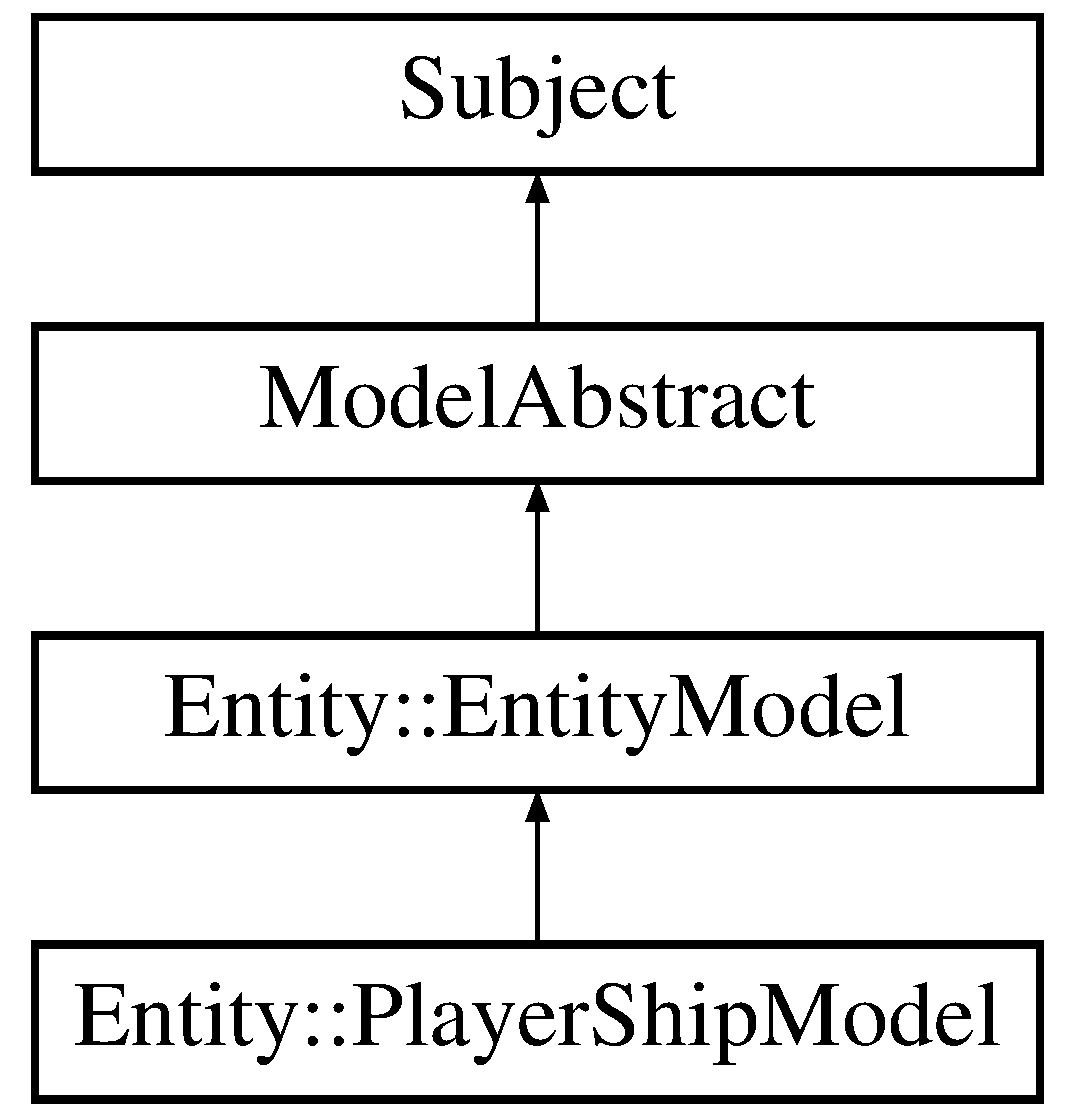
\includegraphics[height=5.000000cm]{classEntity_1_1PlayerShipModel}
\end{center}
\end{figure}
\doxysubsection*{Public Member Functions}
\begin{DoxyCompactItemize}
\item 
\mbox{\Hypertarget{classEntity_1_1PlayerShipModel_ab1562ad33a06d7a0e1a2eb9f72ef61f1}\label{classEntity_1_1PlayerShipModel_ab1562ad33a06d7a0e1a2eb9f72ef61f1}} 
{\bfseries Player\+Ship\+Model} (\mbox{\hyperlink{structUtils_1_1Vector2D}{Utils\+::\+Vector2D}} position, int healthpoints)
\end{DoxyCompactItemize}
\doxysubsection*{Additional Inherited Members}


\doxysubsection{Detailed Description}
Model of the Player\+Ship handles all the data for Player\+Ship. 

Definition at line 13 of file Player\+Ship\+Model.\+h.



The documentation for this class was generated from the following files\+:\begin{DoxyCompactItemize}
\item 
Entity/\+Alive/\+Player\+Ship/Player\+Ship\+Model.\+h\item 
Entity/\+Alive/\+Player\+Ship/Player\+Ship\+Model.\+cpp\end{DoxyCompactItemize}

\hypertarget{classEntity_1_1PlayerShipView}{}\doxysection{Entity\+::Player\+Ship\+View Class Reference}
\label{classEntity_1_1PlayerShipView}\index{Entity::PlayerShipView@{Entity::PlayerShipView}}


View class for Player\+Ship this class handles the visual aspect of the game.  




{\ttfamily \#include $<$Player\+Ship\+View.\+h$>$}

Inheritance diagram for Entity\+::Player\+Ship\+View\+:\begin{figure}[H]
\begin{center}
\leavevmode
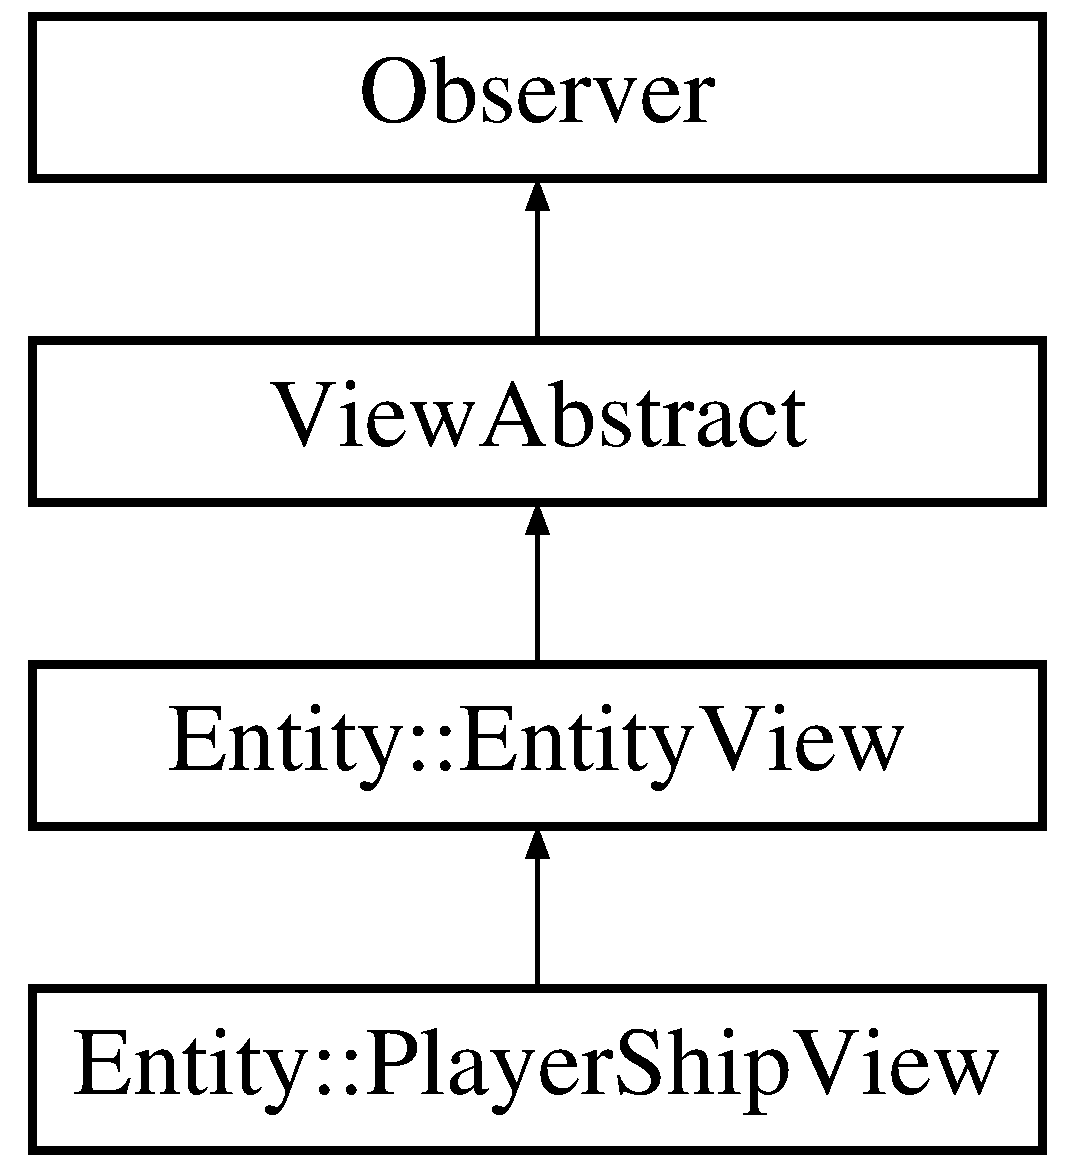
\includegraphics[height=4.000000cm]{classEntity_1_1PlayerShipView}
\end{center}
\end{figure}
\doxysubsection*{Public Member Functions}
\begin{DoxyCompactItemize}
\item 
\mbox{\hyperlink{classEntity_1_1PlayerShipView_a67c871edf52f531bce73dd4e9a0ff34d}{Player\+Ship\+View}} (const std\+::\+\_\+\+\_\+shared\+\_\+ptr$<$ sf\+::\+Render\+Window $>$ \&\mbox{\hyperlink{classViewAbstract_a51b1f37a6113ef3f7b061db29cb4a4c0}{w}}, std\+::weak\+\_\+ptr$<$ \mbox{\hyperlink{classModelAbstract}{Model\+Abstract}} $>$ \mbox{\hyperlink{classEntity_1_1EntityView_a795dc4dd2410feba1a800f7a8b99e09f}{model}})
\begin{DoxyCompactList}\small\item\em the constructor of a playershipview \end{DoxyCompactList}\item 
\mbox{\Hypertarget{classEntity_1_1PlayerShipView_a1a3e9f8b78fc6fbe450b72dc5e39e622}\label{classEntity_1_1PlayerShipView_a1a3e9f8b78fc6fbe450b72dc5e39e622}} 
void \mbox{\hyperlink{classEntity_1_1PlayerShipView_a1a3e9f8b78fc6fbe450b72dc5e39e622}{generate\+Shape}} ()
\begin{DoxyCompactList}\small\item\em generates the drawable for the Playership\+View \end{DoxyCompactList}\end{DoxyCompactItemize}
\doxysubsection*{Public Attributes}
\begin{DoxyCompactItemize}
\item 
\mbox{\Hypertarget{classEntity_1_1PlayerShipView_ad947f6498446c86f9827877059f8871a}\label{classEntity_1_1PlayerShipView_ad947f6498446c86f9827877059f8871a}} 
sf\+::\+Texture \mbox{\hyperlink{classEntity_1_1PlayerShipView_ad947f6498446c86f9827877059f8871a}{texture}}
\begin{DoxyCompactList}\small\item\em The texture that will be drawn on te sf\+::sprite shape. \end{DoxyCompactList}\end{DoxyCompactItemize}
\doxysubsection*{Additional Inherited Members}


\doxysubsection{Detailed Description}
View class for Player\+Ship this class handles the visual aspect of the game. 

Definition at line 13 of file Player\+Ship\+View.\+h.



\doxysubsection{Constructor \& Destructor Documentation}
\mbox{\Hypertarget{classEntity_1_1PlayerShipView_a67c871edf52f531bce73dd4e9a0ff34d}\label{classEntity_1_1PlayerShipView_a67c871edf52f531bce73dd4e9a0ff34d}} 
\index{Entity::PlayerShipView@{Entity::PlayerShipView}!PlayerShipView@{PlayerShipView}}
\index{PlayerShipView@{PlayerShipView}!Entity::PlayerShipView@{Entity::PlayerShipView}}
\doxysubsubsection{\texorpdfstring{PlayerShipView()}{PlayerShipView()}}
{\footnotesize\ttfamily Entity\+::\+Player\+Ship\+View\+::\+Player\+Ship\+View (\begin{DoxyParamCaption}\item[{const std\+::\+\_\+\+\_\+shared\+\_\+ptr$<$ sf\+::\+Render\+Window $>$ \&}]{w,  }\item[{std\+::weak\+\_\+ptr$<$ \mbox{\hyperlink{classModelAbstract}{Model\+Abstract}} $>$}]{model }\end{DoxyParamCaption})}



the constructor of a playershipview 


\begin{DoxyParams}{Parameters}
{\em w} & \\
\hline
{\em model} & \\
\hline
\end{DoxyParams}


Definition at line 15 of file Player\+Ship\+View.\+cpp.


\begin{DoxyCode}{0}
\DoxyCodeLine{15                                                                                                               : \mbox{\hyperlink{classEntity_1_1EntityView_a3f693acc2d87f02562b8613dae88540b}{EntityView}}(\mbox{\hyperlink{classViewAbstract_a51b1f37a6113ef3f7b061db29cb4a4c0}{w}},\mbox{\hyperlink{classEntity_1_1EntityView_a795dc4dd2410feba1a800f7a8b99e09f}{model}}) \{}
\DoxyCodeLine{16         \mbox{\hyperlink{classEntity_1_1PlayerShipView_a1a3e9f8b78fc6fbe450b72dc5e39e622}{generateShape}}();}
\DoxyCodeLine{17 \}}

\end{DoxyCode}


The documentation for this class was generated from the following files\+:\begin{DoxyCompactItemize}
\item 
Entity/\+Collidable/\+Alive/\+Player\+Ship/Player\+Ship\+View.\+h\item 
Entity/\+Collidable/\+Alive/\+Player\+Ship/Player\+Ship\+View.\+cpp\end{DoxyCompactItemize}

\hypertarget{classUtils_1_1StopWatch}{}\doxysection{Utils\+::Stop\+Watch Class Reference}
\label{classUtils_1_1StopWatch}\index{Utils::StopWatch@{Utils::StopWatch}}
\doxysubsection*{Public Member Functions}
\begin{DoxyCompactItemize}
\item 
\mbox{\Hypertarget{classUtils_1_1StopWatch_a6307657657fdea9e3fbd6894f93f3949}\label{classUtils_1_1StopWatch_a6307657657fdea9e3fbd6894f93f3949}} 
void {\bfseries start} ()
\item 
\mbox{\Hypertarget{classUtils_1_1StopWatch_a13136ad8120b345c4d16f7f600867246}\label{classUtils_1_1StopWatch_a13136ad8120b345c4d16f7f600867246}} 
double {\bfseries elapsed} ()
\end{DoxyCompactItemize}
\doxysubsection*{Static Public Member Functions}
\begin{DoxyCompactItemize}
\item 
\mbox{\Hypertarget{classUtils_1_1StopWatch_a17a03335cbdac0082b880a969b59a22f}\label{classUtils_1_1StopWatch_a17a03335cbdac0082b880a969b59a22f}} 
static \mbox{\hyperlink{classUtils_1_1StopWatch}{Stop\+Watch}} \& {\bfseries get\+Instance} ()
\end{DoxyCompactItemize}


\doxysubsection{Detailed Description}


Definition at line 10 of file Stop\+Watch.\+h.



The documentation for this class was generated from the following files\+:\begin{DoxyCompactItemize}
\item 
Utils/Stop\+Watch.\+h\item 
Utils/Stop\+Watch.\+cpp\end{DoxyCompactItemize}

\hypertarget{classSubject}{}\doxysection{Subject Class Reference}
\label{classSubject}\index{Subject@{Subject}}
Inheritance diagram for Subject\+:\begin{figure}[H]
\begin{center}
\leavevmode
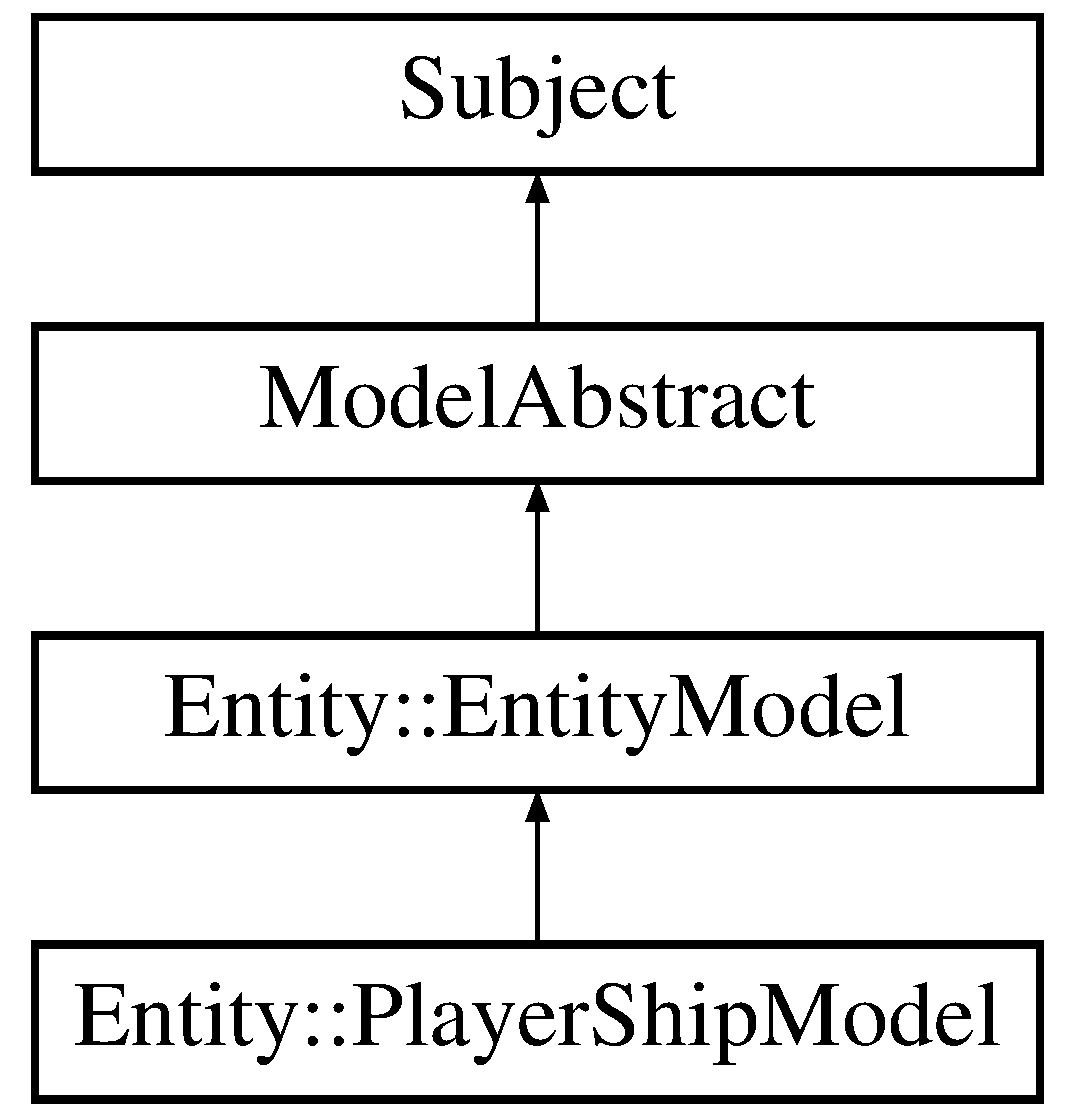
\includegraphics[height=5.000000cm]{classSubject}
\end{center}
\end{figure}
\doxysubsection*{Public Member Functions}
\begin{DoxyCompactItemize}
\item 
\mbox{\Hypertarget{classSubject_ae79704a06089dffc1809c8ac0cd12398}\label{classSubject_ae79704a06089dffc1809c8ac0cd12398}} 
void {\bfseries register\+Observer} (std\+::shared\+\_\+ptr$<$ \mbox{\hyperlink{classObserver}{Observer}} $>$ o)
\item 
\mbox{\Hypertarget{classSubject_ab2b8a1aeb158f75379d3975bc2f96ad0}\label{classSubject_ab2b8a1aeb158f75379d3975bc2f96ad0}} 
void {\bfseries remove\+Observer} (std\+::shared\+\_\+ptr$<$ \mbox{\hyperlink{classObserver}{Observer}} $>$ o)
\item 
\mbox{\Hypertarget{classSubject_aa21e68c3420b0dbbfdbff4f4f0f2e746}\label{classSubject_aa21e68c3420b0dbbfdbff4f4f0f2e746}} 
virtual void {\bfseries notify\+Observers} (double, double)=0
\end{DoxyCompactItemize}
\doxysubsection*{Protected Attributes}
\begin{DoxyCompactItemize}
\item 
\mbox{\Hypertarget{classSubject_ab8b404a56f172645e95d23e86f1b8d95}\label{classSubject_ab8b404a56f172645e95d23e86f1b8d95}} 
std\+::vector$<$ std\+::shared\+\_\+ptr$<$ \mbox{\hyperlink{classObserver}{Observer}} $>$ $>$ {\bfseries observers}
\end{DoxyCompactItemize}


\doxysubsection{Detailed Description}


Definition at line 11 of file Subject.\+h.



The documentation for this class was generated from the following files\+:\begin{DoxyCompactItemize}
\item 
Observer/Subject.\+h\item 
Observer/Subject.\+cpp\end{DoxyCompactItemize}

\hypertarget{classUtils_1_1Transformation}{}\doxysection{Utils\+::Transformation Class Reference}
\label{classUtils_1_1Transformation}\index{Utils::Transformation@{Utils::Transformation}}


used for transforming a models x and y values to the corresponding values on the screen.  




{\ttfamily \#include $<$Transformation.\+h$>$}

\doxysubsection*{Public Member Functions}
\begin{DoxyCompactItemize}
\item 
\mbox{\Hypertarget{classUtils_1_1Transformation_a4c04707895cb31f07f615c6d0dbd6691}\label{classUtils_1_1Transformation_a4c04707895cb31f07f615c6d0dbd6691}} 
double {\bfseries transX} (double, double)
\item 
\mbox{\Hypertarget{classUtils_1_1Transformation_a1b8c8966672f4182309a14b82a5af2cb}\label{classUtils_1_1Transformation_a1b8c8966672f4182309a14b82a5af2cb}} 
double {\bfseries transY} (double, double)
\end{DoxyCompactItemize}
\doxysubsection*{Static Public Member Functions}
\begin{DoxyCompactItemize}
\item 
static \mbox{\hyperlink{classUtils_1_1Transformation}{Transformation}} \& \mbox{\hyperlink{classUtils_1_1Transformation_a03b9f5b948a515ced74861fa154a3ce4}{get\+Instance}} ()
\begin{DoxyCompactList}\small\item\em This is the only way to get a reference to the \mbox{\hyperlink{classUtils_1_1Transformation}{Transformation}} object and there can only exist 1 object of \mbox{\hyperlink{classUtils_1_1Transformation}{Transformation}};. \end{DoxyCompactList}\end{DoxyCompactItemize}


\doxysubsection{Detailed Description}
used for transforming a models x and y values to the corresponding values on the screen. 

Definition at line 12 of file Transformation.\+h.



\doxysubsection{Member Function Documentation}
\mbox{\Hypertarget{classUtils_1_1Transformation_a03b9f5b948a515ced74861fa154a3ce4}\label{classUtils_1_1Transformation_a03b9f5b948a515ced74861fa154a3ce4}} 
\index{Utils::Transformation@{Utils::Transformation}!getInstance@{getInstance}}
\index{getInstance@{getInstance}!Utils::Transformation@{Utils::Transformation}}
\doxysubsubsection{\texorpdfstring{getInstance()}{getInstance()}}
{\footnotesize\ttfamily static \mbox{\hyperlink{classUtils_1_1Transformation}{Transformation}}\& Utils\+::\+Transformation\+::get\+Instance (\begin{DoxyParamCaption}{ }\end{DoxyParamCaption})\hspace{0.3cm}{\ttfamily [inline]}, {\ttfamily [static]}}



This is the only way to get a reference to the \mbox{\hyperlink{classUtils_1_1Transformation}{Transformation}} object and there can only exist 1 object of \mbox{\hyperlink{classUtils_1_1Transformation}{Transformation}};. 

\begin{DoxyReturn}{Returns}
the reference to the \mbox{\hyperlink{classUtils_1_1Transformation}{Transformation}} object 
\end{DoxyReturn}


Definition at line 19 of file Transformation.\+h.


\begin{DoxyCode}{0}
\DoxyCodeLine{19                                             \{}
\DoxyCodeLine{20                 \textcolor{keyword}{static} Transformation    instance; \textcolor{comment}{// Guaranteed to be destroyed.}}
\DoxyCodeLine{21                 \textcolor{comment}{// Instantiated on first use.}}
\DoxyCodeLine{22                 \textcolor{keywordflow}{return} instance;}
\DoxyCodeLine{23         \}}

\end{DoxyCode}


The documentation for this class was generated from the following files\+:\begin{DoxyCompactItemize}
\item 
Utils/Transformation.\+h\item 
Utils/Transformation.\+cpp\end{DoxyCompactItemize}

\hypertarget{classViewAbstract}{}\section{View\+Abstract Class Reference}
\label{classViewAbstract}\index{View\+Abstract@{View\+Abstract}}


superclass of all view classes handles the visual aspect of the game  




{\ttfamily \#include $<$View\+Abstract.\+h$>$}

Inheritance diagram for View\+Abstract\+:\begin{figure}[H]
\begin{center}
\leavevmode
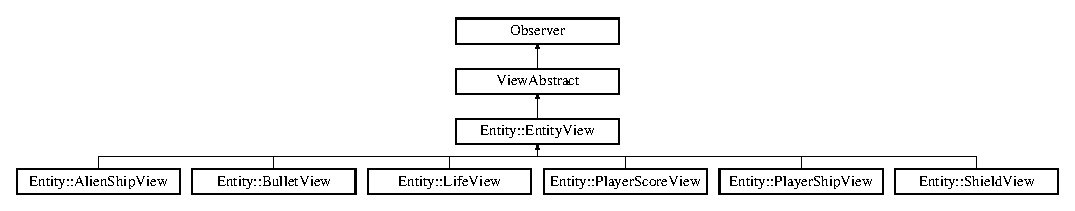
\includegraphics[height=4.000000cm]{classViewAbstract}
\end{center}
\end{figure}
\subsection*{Public Member Functions}
\begin{DoxyCompactItemize}
\item 
\mbox{\Hypertarget{classViewAbstract_ae70e54b453832e601f5332fefb6f4c74}\label{classViewAbstract_ae70e54b453832e601f5332fefb6f4c74}} 
{\bfseries View\+Abstract} (const std\+::\+\_\+\+\_\+shared\+\_\+ptr$<$ sf\+::\+Render\+Window $>$ \&w)
\item 
virtual void \hyperlink{classViewAbstract_ab9d21012b19948e704a800da39b232ba}{draw} (sf\+::\+Render\+Window \&w)=0
\begin{DoxyCompactList}\small\item\em draws a sf\+::\+Drawable on a window \end{DoxyCompactList}\end{DoxyCompactItemize}
\subsection*{Public Attributes}
\begin{DoxyCompactItemize}
\item 
\mbox{\Hypertarget{classViewAbstract_a51b1f37a6113ef3f7b061db29cb4a4c0}\label{classViewAbstract_a51b1f37a6113ef3f7b061db29cb4a4c0}} 
std\+::\+\_\+\+\_\+shared\+\_\+ptr$<$ sf\+::\+Render\+Window $>$ {\bfseries w}
\end{DoxyCompactItemize}


\subsection{Detailed Description}
superclass of all view classes handles the visual aspect of the game 

Definition at line 14 of file View\+Abstract.\+h.



\subsection{Member Function Documentation}
\mbox{\Hypertarget{classViewAbstract_ab9d21012b19948e704a800da39b232ba}\label{classViewAbstract_ab9d21012b19948e704a800da39b232ba}} 
\index{View\+Abstract@{View\+Abstract}!draw@{draw}}
\index{draw@{draw}!View\+Abstract@{View\+Abstract}}
\subsubsection{\texorpdfstring{draw()}{draw()}}
{\footnotesize\ttfamily virtual void View\+Abstract\+::draw (\begin{DoxyParamCaption}\item[{sf\+::\+Render\+Window \&}]{w }\end{DoxyParamCaption})\hspace{0.3cm}{\ttfamily [pure virtual]}}



draws a sf\+::\+Drawable on a window 


\begin{DoxyParams}{Parameters}
{\em w} & the window where the drawable gets drawn on \\
\hline
\end{DoxyParams}


Implemented in \hyperlink{classEntity_1_1EntityView_a9a415b467798f8bbb9cd2489c3edd941}{Entity\+::\+Entity\+View}, \hyperlink{classEntity_1_1PlayerShipView_ad9767510af4af87a4b67182065a1bf6c}{Entity\+::\+Player\+Ship\+View}, and \hyperlink{classEntity_1_1EnemyShipView_a3417632d012f12720ebbbe4b525b3c19}{Entity\+::\+Enemy\+Ship\+View}.



The documentation for this class was generated from the following files\+:\begin{DoxyCompactItemize}
\item 
M\+V\+C\+Abstract/View\+Abstract.\+h\item 
M\+V\+C\+Abstract/View\+Abstract.\+cpp\end{DoxyCompactItemize}

%--- End generated contents ---

% Index
\backmatter
\newpage
\phantomsection
\clearemptydoublepage
\addcontentsline{toc}{chapter}{Index}
\printindex

\end{document}
